\chapter{Introduction} \label{chap:intro}

\section{Motivation}
%\paragraphHead{about data}
%Nowadays, data plays an important role in both academia and business. They can find some
%business opportunities from their data. Then, the field of study that unifies engineering, mathematics, statistics, and computer science emerges, called data science. Data science is broadly
%used in business and industry to find the business opportunity hidden in data. Chatterjee et al. (2021) \cite{...} concluded that using data science in an enterprise increases accuracy in innovative
%decisions and the potentiality of competition in business.
%
%\paragraphHead{Tabular data: a format of data often used and also meet missing (merge to the first paragraph)}
%Tabular data is a format of data that displays in rows and columns.
%One of them corresponds to the collected features of each data sample.
%It is a ubiquitous data format used in practical applications in many domains such as enterprise operations, manufacturing, clinics, and surveys.
%For example, doctors or medical technologists may want to predict the chance of a specific disease for a patient from the patient’s historical records that are stored in the form of a table.
%Missing data problem is also a challenge in modeling tabular data.
%Even though tabular data has its own structure represented by feature vector, missing values can eliminates the structure of tabular data so that model cannot learn or compute on such data.
%%However, one of the efficient approaches that might fill this gap is to represent tabular data by graphs and to use graph neural networks (GNNs).

\paragraphHead{Data Science and Tabular data}
In the contemporary landscape, data holds significant value in academia and business by data-driven paradigm.
It drives the emergence of data science—an interdisciplinary field combining engineering, mathematics, statistics, and computer science.
Applications of data science span various industries, uncovering concealed business opportunities.
Research by Chatterjee et al. (2021) emphasizes its role in enhancing decision accuracy and fostering competitiveness.
Among many kinds of data's format, tabular data is one of the formats that is widespread in domains like healthcare and manufacturing.
It presents a structured means to store information.

\paragraphHead{tell that missing data is a problem often met}
However, not only mining or modeling data but also data preparation is a task that practitioners in data science have to do.
They spend much time in cleaning and organizing data.
One of the common challenges is missing features which is the problem of absence for some values in the given datasets.
This problem is relatively common in almost all research and all formats of data, especially in tabular data.
It can significantly affect results obtained from the data \cite{...} in sense of learning.


\paragraphHead{causes of missing data}
There are many causes of missing data.
First, the problem of measuring instruments is a cause that often occurs in a production line.
Second, some missing data can emerge from the nature of data,
such as different factors corrected between males and females in a clinical survey
or the disappearance of a patient during the treatment process.
Third, the lack of knowledge of the sample can also result in missing data.
There may be the case of the sample giving a ``don't know'' answer to an observer in some complicated question.
Even independence of each measurement process (i.e. each feature) can be considered as a cause of missing data in sense of feature.
That is, some feature can be determined by logical combination of two or more features.
However, independent measurement make such information hidden.

\paragraphHead{significance of missing data}
The missingness problem holds significant importance in machine learning and deep learning, primarily due to its computational implications.
In these fields, including the cutting-edge domain of deep learning, algorithms often rely on fixed-size representation vectors, also known as embeddings.
However, when dealing with missing data without proper preprocessing, a critical challenge arises as data cannot be directly fed into models due to the absence of vital information.
From a theoretical perspective, machine learning involves the search for an optimal distribution within a hypothesis class, guided by a given training dataset.
This search is essentially a quest to find the best model within an equivalent class of models.
However, the presence of missing data complicates this task by weakening the inductive bias of learning; so misleading the learning of models that much more models are equivalent to the model which should be.
In other words, the higher proportion of missing data, the more models in the same equivalence class.
This makes the learning algorithm more difficult to identify and learn the optimal models when working with datasets containing missing values.

%\paragraphHead{Imputation: the most basic solution}
%One of the simple way is to basically impute these missing values by a constant value, mean or interpolation.
%However, these imputation may not reflect the actual dataset.
%Actually, we do not even know the actual dataset.
%In addition, some missing behavior is also informative such as unrating the product from a customer which may mean dissatisfaction but the customer avoids giving a reason directly.
%So imputation seems that we do not concern the hidden information about missing data.
%Moreover, Ma, et al. (2018) \cite{Ma} commented that the imputation method ignores uncertainties of data which means as the same as hidden information said earlier.
%
%\paragraphHead{More a bit Imputation but with learning from data}
%Not only basic imputation methods, but many work also investigated imputation based methods by learning from data.
%However, it still relies on the assumption that all missing values can be replaced as a number.
%But not all missing scenario can be imputed, for example, unrating the product.
%Also the case of some non measurable feature depending on others, the value 0 and a missing value are not equivalent.
%Moreover, these methods is independent from the learning process.
%In other words, the same model may be lead to different way by different imputation methods.
%The only way is to cross test all possible imputation methods to see whether which method is the best one for the desired model.
%This still requires much effort and time-consumption in the process of feature engineering.
%
%\paragraphHead{Imputation: the most basic solution}
%A variety of methods exist for handling missing values, including straightforward approaches like replacing them with constants, means, or using interpolation.
%However, these methods may not accurately represent the true nature of the dataset.
%The challenge arises because the actual dataset is often unknown, and some missing patterns carry valuable information, such as a customer choosing not to rate a product, indicating potential dissatisfaction without specifying the reason.
%Imputation methods, in this context, may overlook the hidden information within missing data.
%Additionally, studies like Ma et al. (2018) \cite{Ma} argue that imputation methods disregard data uncertainties, echoing the earlier notion of hidden information.
%While more advanced imputation methods based on data learning have been explored, they still assume that all missing values can be numerically replaced, which is not always feasible—consider scenarios like product unrated or non-measurable features dependent on others.
%Furthermore, these methods operate independently of the learning process, meaning that the same model may yield different results based on the chosen imputation method.
%Consequently, determining the most suitable imputation method for a specific model often involves extensive cross-testing, demanding considerable effort and time in the feature engineering phase.

\paragraphHead{Brief Literature: existing methods which}
The most basic methods to handle this issue is imputation for the missing values.
Many work also attempts to find methods to impute missing data in various way including distribution-based imputation and learning the missing values as well.

******To the best of our knowledge, there is no state-of-the-art imputation methods.
Even in practice, the casewise deletion, i.e. removing the data points containing missing values, seems to be the most practical method if much more data is available. 

However, Ma et al. (2018) \cite{Ma} argue that imputation methods disregard data uncertainties, echoing the earlier notion of hidden information.
Even in some real-world case, missing values are their native structure which does not make sense to impute with value.





\paragraphHead{Brief Literature: GNN potential}
From the review of literature, we found an interesting framework addressing this issue in different perspective by graph, called GRAPE \cite{GRAPE}.
They proposed a framework that can learn from data containing missing values without imputation for these missing subjects.
GRAPE is a graph-based framework that table of data is represented by a graph which will be processed by an deep-network algorithm call graph neural networks (GNNs).
This demonstrates the potential that representing data by graphs and using GNN algorithms can weaken the need of completeness of datasets.
In other words, GNNs with graph data structure are more flexible in computation rather than using the fixed length of feature vector fed into algorithm directly.

Not only missing data, but GNNs are also used in many works that investigated approaches for modeling complete tabular data. 
There are both an idea of using one graph for the whole table \cite{grape} does and idea of using a dataset of graphs which of each corresponds to each instance of table \cite{...}.
It is a naive idea to use a big graph for the entire table to learn an hidden information inferred between row (instance) or column (feature).
On the other hand, some work uses a graph of instance to capture hidden information inside the instance among its feature value.


\paragraphHead{Brief Literature: Gap between GNN and missing data}
GRAPE is an sample algorithm that allows avoidance of imputation.
It is designed to capture the cooperating information between a node of instance and a node of feature that is observed for the instance and the captured information is aggregated to the node of instance to infer its corresponding label.
Technically, it seems to utilize the flexibility of GNNs to omit the missing feature by not using the information from that feature node.
However, some missing values may be informative in sense of structure.
They should be utilized in prediction, not abandoned.

In contrast, the another idea to represent tabular data by graph, which represents each instance by a graph, is still not explored to address missing issue.
So this motivates us to study how to address the missing data issue by the idea of graphs of samples because we believe that the graph of a sample should be effectively used for capturing dependency of missingness.

To the best of our knowledge, no work address the missing data by this idea.
However, tabular data is not native graph data structure.
So it comes up with the question of how to represent data by graphs and how to design GNN algorithm to process them.

\paragraphHead{How we will fill the gap}
To fill the aforementioned gap, this work proposes the end-to-end GNN framework from tabular data to predicted label.
The framework consists of two major modules: (1) graph construction and (2) prediction from graphs as shown in Figure \ref{framework}.

\begin{figure}[h]
	\centering
	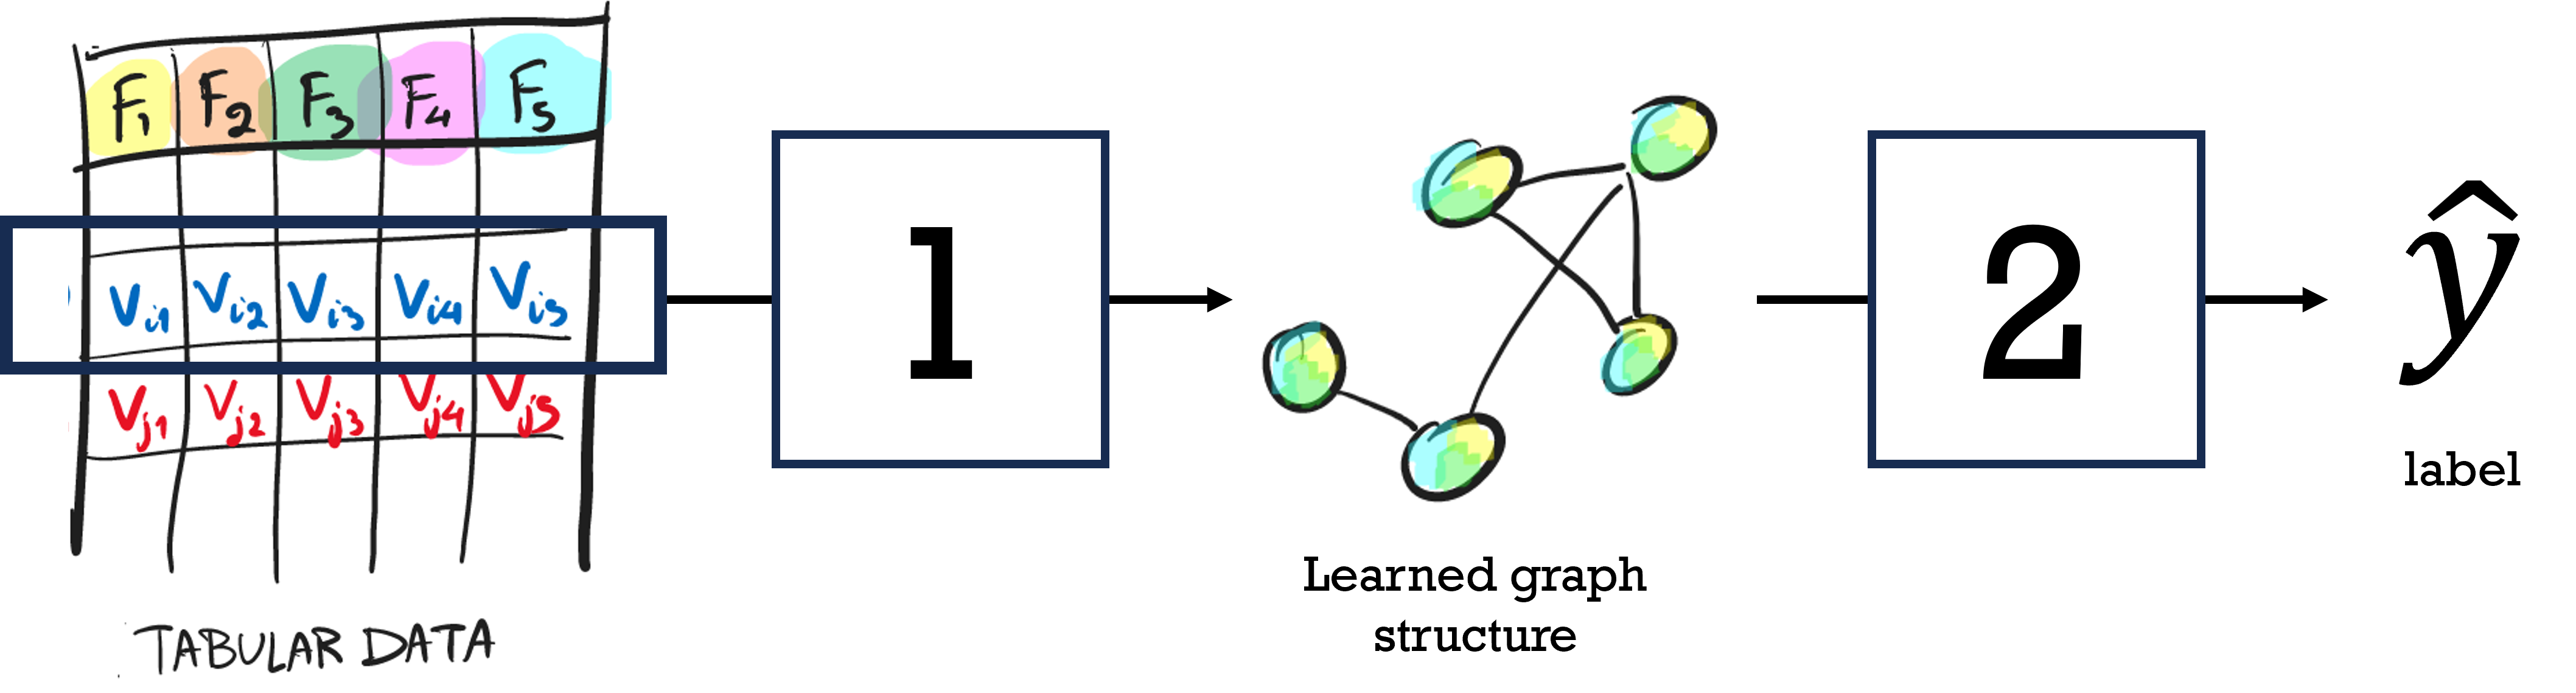
\includegraphics[width=0.7\linewidth]{framework}
	\caption{text}\label{framework}
\end{figure}

% [] want to include idea that complete graph may introduce much noise not related
 
The graph construction module is for learning the structure of a graph of a given data point which is used as a graph representation of the instance.
Since some missing values is caused by dependency of values of other features, e.g. not measurable attribute in male patient, we aim to develop a graph structure learning module so that it can keep dependency between features.
Not only dependency, interaction between feature, i.e. the higher-order nonlinear operation between features is also an interesting characteristic of tabular data that can be considered as a missing value.
Hence we also aim that this module of our work can also keep the interaction information in the learned graph structure.

On the other hand, we then develop the module making prediction from the learned graphs.
This prediction is aimed to be robust for missing values, noise features, dependency and also interaction.


%\paragraphHead{It's time to tell about graphs and GNNs: graph first}
%From the issue of missing data, we need a learning algorithm or a data structure that is more flexible in computation rather than using the fixed length of feature vector fed into algorithm directly.
%This work concentrates on graphs data structures and graph neural network (GNN) algorithms.
%As we have ever seen in data structure, graphs are flexible in how to storage data via edges and nodes.
%Moreover, they are suitable to be flexibly computed by using edges. 
%
%\paragraphHead{It's time to tell about graphs and GNNs: GNNs next}
%GNNs are a class of neural based methods designed to perform inference on graph data.
%It has emerged as a promising approach for modeling structured and semi-structured data, such as social networks \cite{Zhang2019}, molecular structures \cite{Gilmer2017}, and knowledge graphs \cite{Schlichtkrull}.
%Particularly when dealing with high-dimensional or incomplete datasets, GNNs have demonstrated superior performance in various applications, as they effectively capture complex dependencies among nodes and edges in a graph \cite[Kipf \& Welling 2017]{GCN}.
%Moreover, GNNs have advantages over traditional machine learning methods as they do not rely on assumptions about independence of instances and features.
%This makes GNNs are more flexible in learning with respect to both data they use and computation they do.

%\paragraphHead{Conclude to our expectation to use graphs and GNNs to address missing data problem}
%Therefore, the objective of this work is to investigate the new method to learn representations or embeddings of tabular data containing missing values by using GNNs.
%We also aim to find a new way to represent tabular data by a graph.
%The proposed algorithm will allow users to directly feed a data point from tabular data containing missing values without any preprocessing process.
%Moreover, the model can be trained in an end-to-end fashion.

\section{Research Objectives}
%\subsection*{Problem Statement}
%Missing data, which often occurs in many domains of tabular data, can lead to biased or inaccurate models if not handled properly.
%Current methods for handling missing data, such as imputation, can introduce additional assumptions and may not capture the underlying structure of the data.
%Moreover, doing so in the process of feature engineering takes much time and effort of practitioners.
%We seek to develop an approach that can effectively handle missing data in datasets without relying on process of data preparation for missing values such as imputation.
%Our model is also aimed to be able to learn the information of missing values in the sense of natural missing value

%\subsection*{Research Questions}

%\subsection*{Objectives}
The primary objective of this research is to investigate a GNN-based framework that can address the challenge of missing data. The further detail of our objectives is as follows:

\begin{enumerate}
	\item develop an algorithm to construct spare graph structures for the representation of data that can be efficiently used for computation of the corresponding GNN prediction algorithm and maintain the interaction inside the data instance,
	\item develop a GNN algorithm that can be trained by datasets containing missing values without any preprocessing, and also can predict the corresponding label of the given data that may contain missing values.
	\item Validate the developed model both synthetic and real-world datasets.
\end{enumerate}

\section{Outlines}
In Chapter \ref{chap:litrev}, we explain more detail related to our work including graph representation, GNNs and related work.
Readers can find deep detail and also formal definition in the section preliminary of this chapter.
And then, we describe how we perform this research in Chapter \ref{chap:meth}: methodology.

